% 結果の章（数値は 図/values.tex と 図/tab_*.tex から。手で書かない）

% ============================================================
\chapter{主な検定}\label{ch:primary}

\begin{table}[H]
\centering\small
\caption{TE の見積もりの偏り（2015 年末から、四半期ごと、ChronoGPT＋リッジの見通し、\V{primarydays} 日）}
\label{tab:tests}
\begin{tabular}{@{}lrrrrr@{}}
\toprule
比べたもの & $b$（前） & $b$（後） & $D$ & 95\% 区間 & 片側 $p$ \\
\midrule
\textbf{主：C（株価＋テキスト）と B（株価）} & \V{primarybref} & \V{primarybnew} & \V{primaryD} & [\V{primarylo}, \V{primaryhi}] & \V{primaryp} \\
副：B（株価）と A（基準） & \V{BvsAbref} & \V{BvsAbnew} & \V{BvsAD} & [\V{BvsAlo}, \V{BvsAhi}] & \V{BvsAp} \\
副：C（株価＋テキスト）と A（基準） & \V{CvsAbref} & \V{CvsAbnew} & \V{CvsAD} & [\V{CvsAlo}, \V{CvsAhi}] & \V{CvsAp} \\
副：gpt-4o-mini、C と B（2023 年末から、\V{gptCvsBdays} 日） & \V{gptCvsBbref} & \V{gptCvsBbnew} & \V{gptCvsBD} & [\V{gptCvsBlo}, \V{gptCvsBhi}] & \V{gptCvsBp} \\
\bottomrule
\end{tabular}
\end{table}

$b$ は偏りの統計量（日次の超過リターン ÷ 事前の TE の 2 乗平均の平方根。1 なら事前の TE が正しい）。$D = |\log b_{\text{前}}| - |\log b_{\text{後}}|$ が正なら、後の版のほうが 1 に近い。

\begin{keybox}[結果]
主な検定は\textbf{\V{primaryverdict}}。テキストのリスクの点数を足しても、TE の見積もりの偏りはほとんど変わらなかった（$b$ は \V{primarybref} から \V{primarybnew}、片側 $p$ = \V{primaryp}）。一方、副次の検定では、\textbf{株価のデータによる補正（B）が、偏りをはっきり小さくした}（$b$ は \V{BvsAbref} から \V{BvsAbnew}、95\% 区間が 0 を含まない）。
\end{keybox}

\begin{itemize}
\item \textbf{テキストの点数の重み}：C の補正の回帰で学習されたリスクの点数の係数は、リバランスの日の平均で、1 標準偏差あたり変動率の \V{betaC}\%（ChronoGPT）だった。株価のデータの説明変数を入れた補正の回帰の中では、ChronoGPT のリスクの点数にはほとんど重みがつかず、C は B とほぼ同じになった。gpt-4o-mini の点数の係数は \V{betaCgpt}\% だった。
\item \textbf{補正をかけた日の割合}：B は \V{usedB}、C は \V{usedC}、gpt-4o-mini の C は \V{usedCgpt}（学習の発表が足りない日は B の倍率を使った）。
\end{itemize}

% ============================================================
\chapter{すべての組み合わせ}\label{ch:runs}

\section{偏りの統計量}

\begin{figure}[H]
\centering
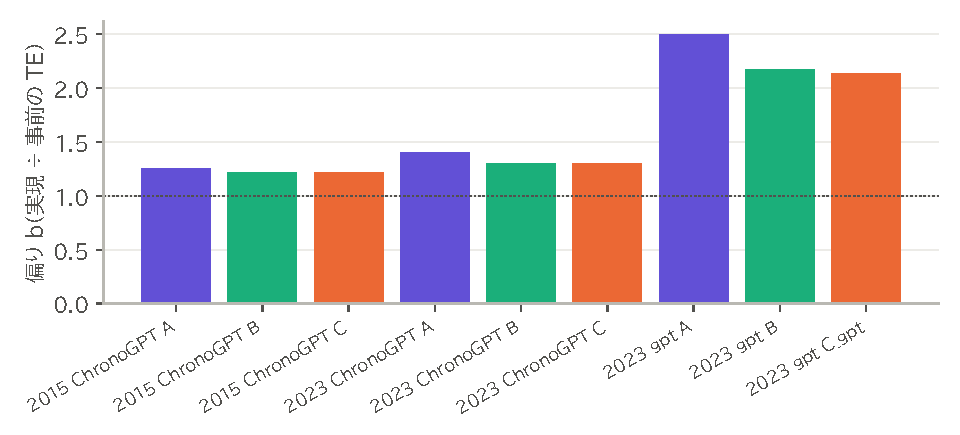
\includegraphics[width=0.8\linewidth]{bias.pdf}
\caption{四半期ごとのリバランスの、版ごとの偏り $b$。点線は 1（事前の TE が正しい）。}
\label{fig:bias}
\end{figure}

\begin{itemize}
\item どの組み合わせでも $b > 1$ で、事前の TE は実現の TE を\textbf{小さく見積もっていた}。S1 の追記 1 で見た「実現の TE が上限を超える」問題が、ここでも確かめられた。
\item 株価による補正（B）は、2015 年末から・2023 年末から、ChronoGPT・gpt-4o-mini の見通し、四半期・半年・1 年のどの組み合わせでも、偏りを A より小さくした（\tabref{tab:runs2015}・\tabref{tab:runs2023}）。テキストを足した C は、B とほとんど同じだった。
\item gpt-4o-mini の見通しの BLM は、偏りが特に大きい（四半期・半年ごとでは $b$ が 2 を超える）。事前の TE は年 2〜3\% だが、四半期・半年ごとでは実現の TE がその 2 倍前後だった。
\end{itemize}

\section{2015 年末から}

\begin{table}[H]
\centering\small
\caption{2015 年 12 月末を 1 とした推移（2026 年 9 月末まで）。年率と相手との差は年率、TE は年率、回転率はリバランス 1 回あたり}
\label{tab:runs2015}
\tabin{runs_2015}
\end{table}

\begin{figure}[H]
\centering
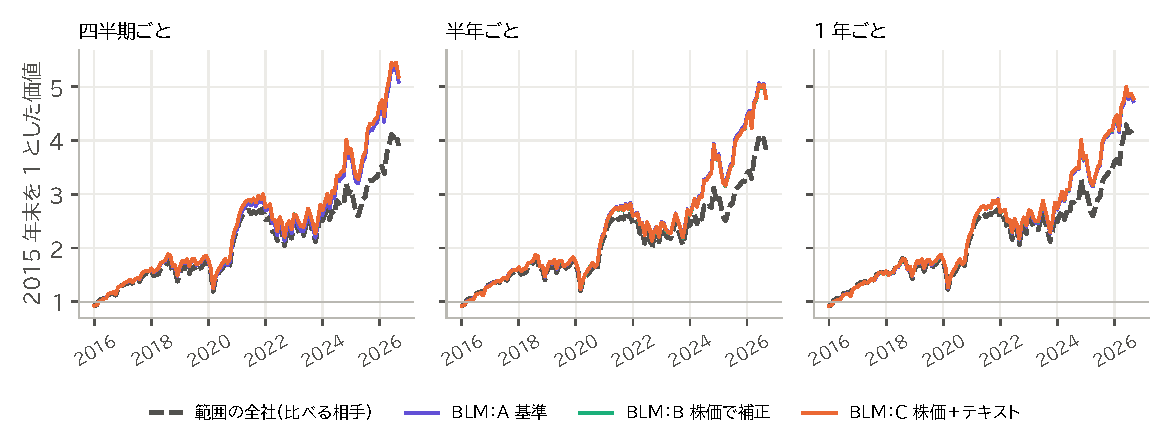
\includegraphics[width=\linewidth]{paths_2015_chrono_ridge.pdf}
\caption{2015 年末を 1 とした推移（ChronoGPT＋リッジの見通し）。3 つの版の線はほぼ重なる。}
\label{fig:paths2015}
\end{figure}

\section{2023 年末から}

\begin{table}[H]
\centering\small
\caption{2023 年 12 月末を 1 とした推移（2026 年 9 月末まで、約 2 年 9 か月）}
\label{tab:runs2023}
\tabin{runs_2023}
\end{table}

\begin{figure}[H]
\centering
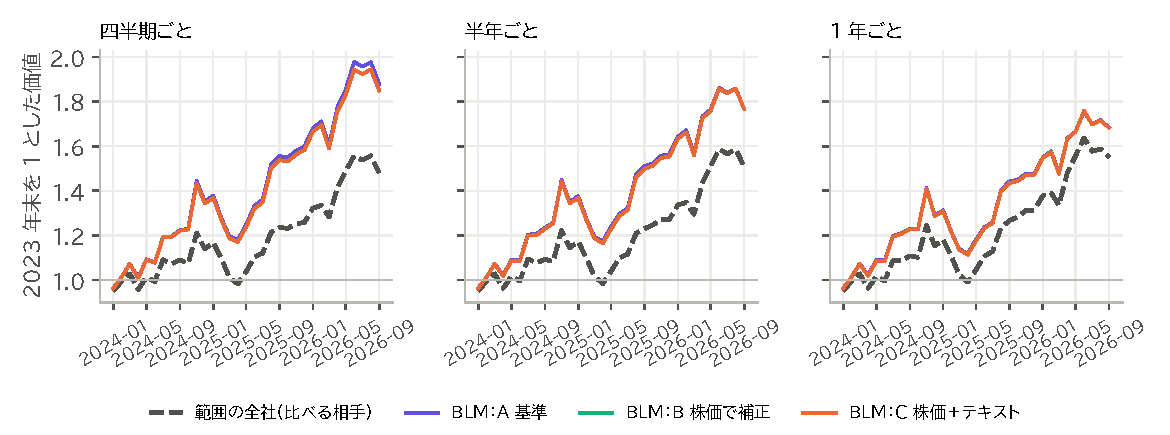
\includegraphics[width=\linewidth]{paths_2023_chrono_ridge.pdf}
\caption{2023 年末を 1 とした推移（ChronoGPT＋リッジの見通し）。}
\label{fig:paths2023c}
\end{figure}

\begin{figure}[H]
\centering
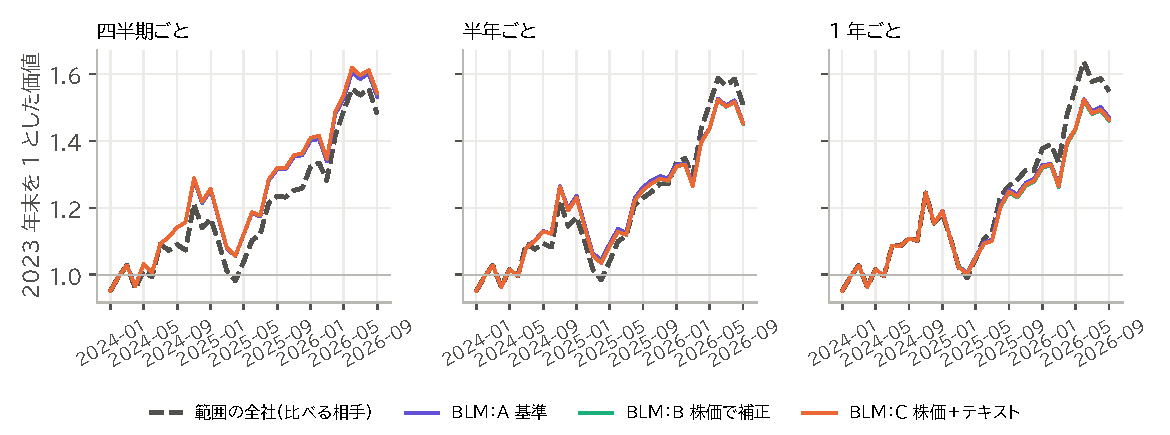
\includegraphics[width=\linewidth]{paths_2023_gpt_ridge.pdf}
\caption{2023 年末を 1 とした推移（gpt-4o-mini（重みを学習）の見通し）。}
\label{fig:paths2023g}
\end{figure}

\begin{itemize}
\item 推移は、3 つの版でほぼ重なった。共分散の補正は、リターンにはほとんど影響しない。2015 年末から四半期ごとでは、最終の値は A が \V{B2015quarterchronoridgeA}、B が \V{B2015quarterchronoridgeB}、C が \V{B2015quarterchronoridgeC}（比べる相手は \V{B2015quarterband}）。
\item ChronoGPT＋リッジの見通しの BLM は、どの版でも、2015 年末から・2023 年末からの両方で、比べる相手を上回った（S1 の追記 1 と同じ）。gpt-4o-mini（重みを学習）の見通しは、四半期ごとではわずかに上回り、半年・1 年ごとでは下回った。
\item 資産の水準は、生存者バイアスで高く出ている。意味があるのは差だけである。
\end{itemize}

% ============================================================
\chapter{解釈}\label{ch:interpret}

\section{何が分かったか}

\begin{enumerate}
\item \textbf{テキストのリスクの点数で共分散を補正しても、BLM のリスクの見積もりは良くならなかった}。S2 で見たテキストの効果は小さく、株価のデータ（発表の前の変動率、2 日の反応の大きさ）と一緒に補正の回帰に入れると、ChronoGPT のリスクの点数にはほとんど重みがつかなかった。S2 の結論（「予測の力はあるが、大きさは小さく、水準の予測には役立たない」）と一致する。
\item \textbf{株価のデータによる補正は、リスクの見積もりをはっきり良くした}。発表の後の銘柄の分散を、直近の変動率と反応の大きさで相対的に補正するだけで、すべての組み合わせで偏りが小さくなった。決算の後のリスクの変化は、直近 252 日の共分散では捉えきれない。
\item \textbf{それでも事前の TE は小さすぎる}。補正しても $b$ は ChronoGPT の見通しで 1.2〜1.5、gpt-4o-mini の見通しで 1.4〜2.3 で、実現の TE は事前の上限を 2 割以上超えた。最適化は、推定の誤差で小さく見積もられたリスクの方向に比率を寄せやすい（平均分散の「誤差の最大化」、ヘッジファンドの報告書の第 7 章）。共分散の推定（500 銘柄前後を 252 日で）の誤差と、小型株の固有の変動の急な変化が、その原因の候補である。
\item \textbf{推移はほとんど変わらなかった}。共分散の補正は、TE の配分を少し動かすだけで、リターンの大きさは見通しで決まる。
\end{enumerate}

\section{次に試すこと}

\begin{itemize}
\item \textbf{TE の校正}：過去の偏り $b$ で事前の TE の上限を割り引く（実験 X03 の考え方。上限 3\% なら、$b = 1.2$ のとき事前の上限を 2.5\% にする）。
\item \textbf{共分散の推定}：ファクター型のリスクモデル（業種・規模・モメンタムなど）や、より強い縮小。株価による補正（B）は残す。
\item \textbf{gpt-4o-mini の見通しの偏りの理由}：見通しがどの銘柄・どのリスクに偏っているかを調べる（探索）。
\item \textbf{テキストのリスクの点数}は、共分散の補正ではなく、S2 で効いた「2 日の反応の大きさ」の予測（決算の前後の量の調整）に使う方が筋がよいかもしれない。
\end{itemize}
